%%%%%%%%%%%%%%%%%%%%%%%%%%%%%%%%%%%%%%%%%
% Classicthesis Typographic Thesis
% LaTeX Template
% Version 1.3 (15/2/14)
%
% This template has been downloaded from:
% http://www.LaTeXTemplates.com
%
% Original author:
% André Miede (http://www.miede.de)
%
% License:
% CC BY-NC-SA 3.0 (http://creativecommons.org/licenses/by-nc-sa/3.0/)
%
% General Tips:
% 1) Make sure to edit the classicthesis-config.file
% 2) New enumeration (A., B., C., etc in small caps): \begin{aenumerate} \end{aenumerate}
% 3) For margin notes: \marginpar or \graffito{}
% 4) Do not use bold fonts in this style, it is designed around them
% 5) Use tables as in the examples
% 6) See classicthesis-preamble.sty for useful commands
%
%%%%%%%%%%%%%%%%%%%%%%%%%%%%%%%%%%%%%%%%%

%----------------------------------------------------------------------------------------
%	PACKAGES AND OTHER DOCUMENT CONFIGURATIONS
%----------------------------------------------------------------------------------------

\documentclass[
		twoside,openright,titlepage,numbers=noenddot,headinclude,1headlines,
                footinclude=true,cleardoublepage=empty,
                BCOR=5mm,paper=a4,fontsize=11pt, % Binding correction, paper type
                american, % Languages
                ]{scrreprt}

% Includes the file which contains all the document configurations and packages
% - make sure to edit this file

\input{tex/classicthesis-config}
% use upquote if available, for straight quotes in verbatim environments
\IfFileExists{upquote.sty}{\usepackage{upquote}}{}
% use microtype if available
\IfFileExists{microtype.sty}{\usepackage{microtype}}{}
\usepackage{biblatex}
\usepackage{color}
\usepackage{fancyvrb}
\newcommand{\VerbBar}{|}
\newcommand{\VERB}{\Verb[commandchars=\\\{\}]}
\DefineVerbatimEnvironment{Highlighting}{Verbatim}{commandchars=\\\{\},fontsize=\small}
% Add ',fontsize=\small' for more characters per line
\usepackage{framed}
\definecolor{shadecolor}{RGB}{248,248,248}
\newenvironment{Shaded}{\begin{snugshade}}{\end{snugshade}}
\newcommand{\KeywordTok}[1]{\textcolor[rgb]{0.13,0.29,0.53}{\textbf{{#1}}}}
\newcommand{\DataTypeTok}[1]{\textcolor[rgb]{0.13,0.29,0.53}{{#1}}}
\newcommand{\DecValTok}[1]{\textcolor[rgb]{0.00,0.00,0.81}{{#1}}}
\newcommand{\BaseNTok}[1]{\textcolor[rgb]{0.00,0.00,0.81}{{#1}}}
\newcommand{\FloatTok}[1]{\textcolor[rgb]{0.00,0.00,0.81}{{#1}}}
\newcommand{\CharTok}[1]{\textcolor[rgb]{0.31,0.60,0.02}{{#1}}}
\newcommand{\StringTok}[1]{\textcolor[rgb]{0.31,0.60,0.02}{{#1}}}
\newcommand{\CommentTok}[1]{\textcolor[rgb]{0.56,0.35,0.01}{\textit{{#1}}}}
\newcommand{\OtherTok}[1]{\textcolor[rgb]{0.56,0.35,0.01}{{#1}}}
\newcommand{\AlertTok}[1]{\textcolor[rgb]{0.94,0.16,0.16}{{#1}}}
\newcommand{\FunctionTok}[1]{\textcolor[rgb]{0.00,0.00,0.00}{{#1}}}
\newcommand{\RegionMarkerTok}[1]{{#1}}
\newcommand{\ErrorTok}[1]{\textbf{{#1}}}
\newcommand{\NormalTok}[1]{{#1}}

% prevent graphics from overflowing
\usepackage{graphicx}
\makeatletter
\def\maxwidth{\ifdim\Gin@nat@width>\linewidth\linewidth\else\Gin@nat@width\fi}
\def\maxheight{\ifdim\Gin@nat@height>\textheight\textheight\else\Gin@nat@height\fi}
\makeatother
\setkeys{Gin}{width=\maxwidth,height=\maxheight,keepaspectratio}

%%%%%%%%%% Version 1.0 %%%%%%%%%%

% Model:
% \newcommand{\nDomains}{D}
% \newcommand{\indexDomain}{i}
% \newcommand{\directStat}{y}
% \newcommand{\directStatIndexed}{y_{\indexDomain}}
% \newcommand{\trueStat}{\mu}
% \newcommand{\trueStatIndexed}{\mu_{\indexDomain}}
% \newcommand{\indexUnit}{j}
% \newcommand{\nUnitIndexed}{n_\indexDomain}

% Sampling-Error
% \newcommand{\samplingError}{e}
% \newcommand{\samplingErrorIndexed}{e_{\indexDomain}}
% \newcommand{\samplingErrorUnitIndexed}{e_{\indexDomain\indexUnit}}
% \newcommand{\samplingVariance}{\sigma_e^2}
% \newcommand{\samplingVarianceIndexed}{\sigma_{e, i}^2}
% \newcommand{\samplingSD}{\sigma_e}
%
% % Uni Error
% \newcommand{\unitError}{e}
%
% % Random Effects
% \newcommand{\randomEffectIndexed}{v_{\indexDomain}}
% \newcommand{\randomEffect}{v}
% \newcommand{\randomEffectVariance}{\sigma_v^2}
% \newcommand{\randomEffectSD}{\sigma_v}
% \newcommand{\RandomEffect}{\mathbf{v}}

% Regressors
% \newcommand{\xArea}{x_{\indexDomain}}
% \newcommand{\xUnit}{x_{\indexDomain\indexUnit}}
% \newcommand{\X}{\mathbf{X}}
% \newcommand{\indexRegressor}{p}
% \newcommand{\nRegressor}{P}

% Math Operators
% \DeclareMathOperator{\tr}{tr}
% \DeclareMathOperator{\diag}{diag}

% Matrix Notation
% \newcommand{\IdentityMatrix}{\mathbf{I}}


% Fixed Point
\newcommand{\aFH}{\psi(\mathbf{r})^\top \mathbf{U}^{\frac{1}{2}}\mathbf{V}^{-1}\frac{\partial\mathbf{V}}{\partial\theta}\mathbf{V}^{-1}\mathbf{U}^{\frac{1}{2}} \psi(\mathbf{r})}


%%%%%%%%%% Version 2.0 %%%%%%%%%%
% constants:

\newcommand{\sige}{\sigma_{ei}^2}
\newcommand{\sigre}{\sigma_{u}^2}
\newcommand{\re}{u}
\newcommand{\half}{\frac{1}{2}}

% funs:
\DeclareMathOperator{\tr}{tr}
\newcommand{\Tr}[1]{tr\left(#1\right)}
\DeclareMathOperator{\diag}{diag}
\newcommand{\Diag}[1]{diag\left(#1\right)}
\newcommand{\Paran}[1]{\left(#1\right)}

% formats:
\newcommand{\Distr}[1]{\mathcal{#1}}
\newcommand{\mat}[1]{\mathbf{#1}}
\newcommand{\pmat}[1]{\boldsymbol{#1}}
\newcommand{\Exp}[1]{\mathbb{#1}}

% subscripts:
\newcommand{\si}[1]{#1_i}
\newcommand{\sij}[1]{#1_{ij}}

% references
\newcommand{\eq}[1]{(\ref{#1})}

\newcommand{\textrrmse}{Boxplot with Relative Root Mean Squared Error (RRMSE)}
\newcommand{\textrbias}{Boxplot with Relative Bias (RBIAS)}


\begin{document}

\frenchspacing % Reduces space after periods to make text more compact

\raggedbottom % Makes all pages the height of the text on that page

\selectlanguage{american} % Select your default language - e.g. american or ngerman

%\renewcommand*{\bibname}{new name} % Uncomment to change the name of the bibliography
%\setbibpreamble{} % Uncomment to include a preamble to the bibliography - some text before the reference list starts

\pagenumbering{roman} % Roman page numbering prior to the start of the thesis content (i, ii, iii, etc)

\pagestyle{plain} % Suppress headers for the pre-content pages

%-------------------------------------------------------------------------------
%	PRE-CONTENT THESIS PAGES
%-------------------------------------------------------------------------------

% Title Page

\begin{titlepage}

\begin{addmargin}[-1cm]{-3cm}
\begin{center}
\large

\hfill
\vfill

\begingroup
\color{Maroon}
\spacedallcaps{\myTitlei} \\  % Thesis title
\spacedallcaps{\myTitleii} \\
\medskip
\endgroup

\spacedlowsmallcaps{\mySubtitle}

\bigskip

\spacedlowsmallcaps{\myName} % Your name

\vfill

%\includegraphics[width=6cm]{figs/FULogo_RGB} \\ \medskip % Picture

% \\ \medskip % Thesis subtitle
\myDegree \\
% \myDepartment \\
\myFaculty \\
\myUni \\ \bigskip

\myTime\ -- \myVersion % Time and version

\vfill

\end{center}
\end{addmargin}

\end{titlepage}
 % Main title page

%\include{tex/Titleback} % Back of the title page

%\cleardoublepage\include{tex/Dedication} % Dedication page

%\cleardoublepage\include{FrontBackMatter/Foreword} % Uncomment and create a Foreword.tex to include a foreword

%\cleardoublepage% Abstract

\pdfbookmark[1]{Abstract}{Abstract} % Bookmark name visible in a PDF viewer

\begingroup
\let\clearpage\relax
\let\cleardoublepage\relax
\let\cleardoublepage\relax

\chapter{Abstract} % Abstract name

Short summary of the contents\dots

\endgroup

\vfill
\pagebreak

% Zusammenfassung

\pdfbookmark[1]{Zusammenfassung}{Zusammenfassung} % Bookmark name visible in a PDF viewer

\begingroup
\let\clearpage\relax
\let\cleardoublepage\relax
\let\cleardoublepage\relax

\chapter{Zusammenfassung} % Abstract name
\selectlanguage{ngerman}

Kurze Zusammenfassung\dots

\endgroup

\vfill

\selectlanguage{british}
 % Abstract page

%\cleardoublepage% Publications - a page listing research articles written using content in the thesis

\pdfbookmark[1]{Publications}{Publications} % Bookmark name visible in a PDF viewer

\chapter*{Publications} % Publications page text

Some ideas and figures have appeared previously in the following publication:

\bigskip

\noindent Warnholz, S. and T. Schmid (2016). “Simulation Tools for Small Area
Estimation: Introducing the R-package saeSim”. In: \textit{Austrian Journal
of Statistics} 45.1, pp. 55–69.

\bigskip

\noindent The results of this Article are the subject matter of Chapter
\ref{chap:saeSim}. There I state, again, explicitly that these results have been
previously published and how I intend to use them in the context of this Thesis.
 % Publications from the thesis page

%\cleardoublepage\include{tex/Acknowledgments} % Acknowledgements page

\pagestyle{scrheadings} % Show chapter titles as headings

\cleardoublepage\include{tex/Contents} % Contents, list of figures/tables/listings and acronyms

\cleardoublepage

\pagenumbering{arabic} % Arabic page numbering for thesis content (1, 2, 3, etc)
%\setcounter{page}{90} % Uncomment to manually start the page counter at an arbitrary value (for example if you wish to count the pre-content pages in the page count)

\cleardoublepage % Avoids problems with pdfbookmark

%----------------------------------------------------------------------------------------
%	THESIS CONTENT - CHAPTERS
%----------------------------------------------------------------------------------------

%\ctparttext{You can put some informational part preamble text here.} % Text on the Part 1 page describing  the content in Part 1

%\part{Some Kind of Manual} % First part of the thesis

%\include{tex/Chapter01} % Chapter 1

%\cleardoublepage % Empty page before the start of the next part

%------------------------------------------------

\ctparttext{This is the chapter where I want to present the theoretical concepts underpinning the development of software and application. Most notably is the robust version of a Fay-Herriot Type model with different variance-covariance structures.} % Text on the Part 2 page describing the content in Part 2

\part{Theory}

\chapter{Methods in Small Area Estimation}
\section{Unit-Level Models}
\section{Area Level Models}\label{area-level-models}

\subsection{The Fay Herriot Model}\label{the-fay-herriot-model}

The model is introduced by \textcite{Fay79} and is used in small area
estimation for research on area-level. It is build on a sampling model:
\[
\directStat_{\indexDomain} = \trueStat_{\indexDomain} + \samplingError_{\indexDomain},
\] where $\directStat_{\indexDomain}$ is a direct estimator of a
statistic of interest $\trueStat_{\indexDomain}$ for an area
$\indexDomain$ with $\indexDomain = 1, \dots, \nDomains$ and $\nDomains$
being the total number of areas. The sampling error
$\samplingError_{\indexDomain}$ is assumed to be independent and
normally distributed with known variances $\samplingVarianceIndexed$,
i.e.
$\samplingError_{\indexDomain}|\trueStat_{\indexDomain} \sim \mathit{N}(0, \samplingVarianceIndexed)$.
The model is modified with the linking model by assuming a linear
relationship between the true area statistic $\trueStat_{\indexDomain}$
and some auxiliary variables $\xArea$: \[
\trueStat_{\indexDomain} = \xArea^\top \beta + \randomEffectIndexed\text{, } \indexDomain=1,\dots, \nDomains.
\] Note that $\xArea$ is a vector containing area-level (aggregated)
information for $\nRegressor$ variables and $\beta$ is a vector
($1\times \nRegressor$) of regression coefficients describing the
(linear) relationship. The model errors $\randomEffectIndexed$ are
assumed to be independent and normally distributed, i.e.
$\randomEffectIndexed \sim \mathit{N}(0, \randomEffectVariance)$
furthermore $\samplingErrorIndexed$ and $\randomEffectIndexed$ are
assumed to be independent. Combining the sampling and linking model
leads to:

\begin{align}
\label{eq:FH}
\directStatIndexed = \xArea^\top \beta + \randomEffectIndexed + \samplingErrorIndexed.
\end{align}

\input{Rmd/theory_compare_unit_and_area}
\subsection{Spatio-Temporal Fay Harriot
model}\label{spatio-temporal-fay-harriot-model}

The model stated in equation \ref{eq:FH} has been modified for including
historical information by modelling autocorrelated model errors and also
by allowing for spatial correlation (in the model error). See the
discussion in \textcite{Mar13} for more details. \textcite{Mar13} allow
for both spatial and temporal correlation in the model errors. Hence the
sampling model is (simply) extended to include historical information:
\[
y_{dt} = \mu_{dt} + e_{dt},
\] with $d = 1, \dots, D$ and $t = 1, \dots, T$ where $D$ and $T$ are
the total number of areas and time periods respectively. Here
$e_{dt} \sim \mathit{N}(0, \sigma^2_{dt})$ are independent with known
variances $\sigma_{dt}^2$. The model error is composed of a spatial
autoregressive process of order 1 (SAR(1)) and an autoregressive process
of order 1 (AR(1)): \[
\mu_{dt} = x^\top_{dt}\beta + u_{1d} + u_{2dt},
\] where $u_{1d}$ and $u_{2dt}$ follow a SAR(1) and AR(1) respectively:
\[
u_{1d} = \rho_1 \sum_{l\neq d}w_{d,l} u_{1l} + \epsilon_{1d},
\] where $|\rho_1| < 1$ and
$\epsilon_{1d} \sim \mathit{N}(0, \sigma_1^2)$ are i.i.d. with
$d = 1,\dots, D$. $w_{d, l}$ are the elements of $W$ which is the row
standardized proximity matrix $W^0$. The elements in $W^0$ are equal to
1 if areas are neighboured and 0 otherwise (an area is not neighboured
with itself) - thus the dimension of $W^0$ is $D\times D$. As stated
above $u_{2dt}$ follows an AR(1): \[
u_{2dt} = \rho_2 u_{2d, t-1} + \epsilon_{2dt},
\] where $|\rho_2| < 1$ and
$\epsilon_{2dt} \sim \mathit{N}(0, \sigma_2^2)$ are i.i.d. with
$d = 1, \dots, D$ and $t = 1, \dots, T$. Note that $u_{1d}$ and
$u_{2dt}$ and $e_{dt}$ are independent and the sampling error variance
parameters are assumed to be known. The model can then be stated as: \[
\mathbf{y} = \mathbf{X}\beta + \mathbf{Z}\mathbf{u} + \mathbf{e},
\] where $\mathbf{y}$ is the $DT\times 1$ vector containing $y_{dt}$ as
elements, $\mathbf{X}$ is the $DT \times p$ design matrix containing the
vectors $x^\top_{dt}$ as rows, $\mathbf{u}$ is the $(D + DT) \times 1$
vector of model errors and $\mathbf{e}$ the $DT \times 1$ vector of
sampling errors $e_{dt}$. Note that $\mathbf{u} = (u_1^\top, u_2^\top)$
where the $D\times 1$ vector $u_1$ and $DT \times 1$ vector $u_2$ have
$u_{1d}$ and $u_{2dt}$ as elements respectively. Furthermore
$\mathbf{Z} = (\mathbf{Z}_1, \mathbf{Z}_2)$ has dimension
$DT \times (D+DT)$, where
$\mathbf{Z}_1 = \mathbf{I}_D \otimes \mathbf{1}_T$ ($\mathbf{I}_D$
denotes a $D\times D$ identity matrix and $\mathbf{1}_T$ a $1 \times T$
vector of ones) has dimension $DT \times D$ and $\mathbf{Z}_2$ is a
$DT \times DT$ identity matrix.

Concerning the variance of $\mathbf{y}$ first consider the distributions
of all error components.
$\mathbf{e} \sim \mathit{N}(\mathbf{0}, \mathbf{V}_e)$ where
$\mathbf{V}_e$ is a diagonal matrix with the known $\sigma^2_{dt}$ on
the main diagonal.
$\mathbf{u} \sim \mathit{N}(\mathbf{0}, \mathbf{V}_u(\theta))$ with the
block diagonal covariance matrix
$\mathbf{V}_u(\theta) = \text{diag}(\sigma_1^2\Omega_1(\rho_1), \sigma_2^2\Omega_2(\rho_2))$
where $\theta = (\sigma_1^2, \rho_1, \sigma_2^2, \rho_2)$.

\[
\Omega_1(\rho_1) = \left((\mathbf{I}_D - \rho_1\mathbf{W})^\top (\mathbf{I}_D - \rho_1\mathbf{W})\right)^{-1}
\] and follows from the SAR(1) process in the model errors.
$\Omega_2(\rho_2)$ has a block diagonal structure with
$\Omega_{2d}(\rho_2)$ denoting the blocks where the definition of
$\Omega_{2d}(\rho_2)$ follows from the AR(1) process: \[
    \Omega_{2d}(\rho_2) = \frac{1}{1-\rho_2^2}
    \left(
      \begin{matrix}
      1 & \rho_2 & \cdots & \rho_2^{T-2}& \rho_2^{T-1}\\
      \rho_2 & 1 & & & \rho_2^{T-2} \\
      \vdots & & \ddots & & \vdots \\
      \rho_2^{T-2} &&& 1 & \rho_2 \\
      \rho_2^{T-1} & \rho_2^{T-2} & \cdots & \rho_2 & 1\\
      \end{matrix}
      \right)_{T\times T}
  \] The variance of $\mathbf{y}$ can thus be stated as: \[
\mathbb{V}(\mathbf{y}) = \mathbf{V}(\theta) = \mathbf{Z}\mathbf{V}_u(\theta)\mathbf{Z}^\top + \mathbf{V}_e
\] The BLUE of $\beta$ and BLUP of $\theta$ can be stated as
\citep[see][]{Hen75}: \[
\tilde{\beta}(\theta) = \left(\mathbf{X}^\top \mathbf{V}^{-1}(\theta) \mathbf{X} \right)^{-1} \mathbf{X}^\top \mathbf{V}^{-1}(\theta) \mathbf{y}
\] \[
\tilde{u}(\theta) = \mathbf{V}_u(\theta) \mathbf{Z}^\top \mathbf{V}^{-1}(\theta) \left(\mathbf{y} - \mathbf{X}\tilde{\beta}(\theta)\right)
\] Hence the BLUP of $u_1$ and $u_2$ can be stated as: \[
\tilde{u}_1(\theta) = \sigma_1^2 \Omega_1(\rho_1) \mathbf{Z}^\top \mathbf{V}^{-1}(\theta) \left(\mathbf{y} - \mathbf{X}\tilde{\beta}(\theta)\right)
\] \[
\tilde{u}_2(\theta) = \sigma_2^2 \Omega_2(\rho_2) \mathbf{Z}^\top \mathbf{V}^{-1}(\theta) \left(\mathbf{y} - \mathbf{X}\tilde{\beta}(\theta)\right)
\] Estimating $\theta$ leads to the EBLUE for $\beta$ and EBLUPs for
$u_1$ and $u_2$, hence an predictor for the area characteristic
$\mu_{dt}$ is given by: \[
\hat{\mu}_{dt} = x_{dt}^\top \hat{\beta} + \hat{u}_{1d} + \hat{u}_{2dt}
\] \textcite{Mar13} use a restricted maximum likelihood method to
estimate $\theta$ independently of $\beta$. An open question is if this
approach can be applied for the robust spatio-temporal model. Thus we
will continue with the discussion of robust small area methods.


\chapter{Review of Robust Methods in Small Area Estimation}
\subsection{Robust ML Score Functions}\label{robust-ml-score-functions}

\textcite{Fel86} studied the robust estimation of linear mixed model
parameters. However, the proposed approach is based on given variance
parameters $\theta$ which is why \textcite{Sin09} propose an estimation
procedure in which robust estimators for $\beta$ and $\theta$ are solved
iteratively. With given robust estimates for $\beta$ and $\theta$ the
estimation of the random effects is straight forward, the main concern,
however, lies with the estimation of robust variance parameters.
Starting from a mixed model: \[
\mat{y} = \mat{X} \beta + \mat{Z} \re + \mat{e}
\] where $\mat{y}$ is the response vector with elements $y_i$, $\mat{X}$
the design matrix, $\re$ the vector of random effects and $\mat{e}$ the
vector of sampling errors. Both error components are assumed to be
normally distributed with $\mat{\re} \sim \Distr{N}(0, \mat{G})$ and
$\mat{e} \sim \Distr{N}(0, \mat{R})$ where $\mat{G}$ and $\mat{R}$
typically depend on some variance parameters $\theta$. Thus the variance
of y is given by
$\mat{V}(\mat{y}) = \mat{V}(\theta) = \mat{Z}\mat{G}\mat{Z}^\top + \mat{R}$.
Maximizing the likelihood of $\mat{y}$ with respect to $\beta$ and
$\theta$ leads to the following equations:

\begin{align*}
\mat{X}^\top\mat{V}^{-1}\left(\mat{y}-\mat{X}\beta\right) =& 0 \\
\left(\mat{y} - \mat{X}\beta\right)^\top\mat{V}^{-1}          %(y-Xb)'V^-1
\frac{\partial\mat{V}}{\partial\theta_l}                      % dV/dx
\mat{V}^{-1}\left(\mat{y} - \mat{X}\beta\right) -             %V^-1 (y-Xb)
\tr\left(\mat{V}^{-1}\frac{\partial\mat{V}}{\partial\theta_l}\right) =& 0
\end{align*}

where $q$ denotes the number of unknown variance parameters with
$l = 1, \dots, q$. Solving the above equations leads to the ML-estimates
for $\beta$ and $\theta$. To robustify against outliers in the response
variable, the residuals $\left(\mat{y}-\mat{X}\beta\right)$ are
standardized and restricted by some influence function $\psi(\cdot)$.
The standardized residuals are given by \[
\mat{r} = \mat{U}^{-\frac{1}{2}}
\left(\mat{y}-\mat{X}\beta\right)
\] where $\mat{U}$ is the matrix of diagonal elements of $\mat{V}$ and
thus also depends on the variance parameters $\theta$. A typical choice
for $\psi(\cdot)$ is Hubers influence function: \[
\psi(u) = u \min\left(1, \frac{b}{|u|}\right).
\] A typical choice for $b$ is 1.345. The vector of robustified
residuals is denoted by
$\mat{\psi}(\mat{r}) = (\psi(r_1), \dots, \psi(r_{n}))$. Solving the
following robust ML-equations leads to robustified estimators for
$\beta$ and $\theta$:

\begin{align}
\label{eq:rml_beta}
\mat{X}^\top\mat{V}^{-1} \mat{U}^{\frac{1}{2}} \psi(\mat{r}) =& 0 \\
\label{eq:rml_theta}
\Phi_l(\theta) = \psi(\mat{r})^\top\mat{U}^{\frac{1}{2}}\mat{V}^{-1}
\frac{\partial\mat{V}}{\partial\theta_l}
\mat{V}^{-1}\mat{U}^{\frac{1}{2}} \psi(\mat{r}) - \tr\left(K\mat{V}^{-1}\frac{\partial\mat{V}}{\partial\theta_l}\right) =& 0 
\end{align}

where $K$ is a diagonal matrix of the same order as $\mat{V}$ with
diagonal elements $c = \Exp{E}[\psi^2(r)|b]$ where $r$ follows a
standard normal distribution.

\subsubsection{Pseudo Linearization}\label{pseudo-linearization}

This is the representation of the pseudo linear representation of the FH
model. As it is introduced in \textcite{Cha11} and \textcite{Cha14}.

Presenting the FH in pseudo linear form means to present the area means
as a weighted sum of the response vector $y$. The FH model is given by

\begin{align}
\theta_i = \gamma_i y_i + (1 - \gamma_i) x_i^\top \beta 
\end{align}

where $\gamma_i = \frac{\sigma^2_u}{\sigma^2_u + \sigma^2_e}$, so it can
be represented as

\[
\theta_i = w_i^\top y
\]

where

\[
w_i^\top = \gamma_i \mathbf{I}^\top_i + (1 - \gamma_i) x_i^\top \mathbf{A}
\]

and

\[
\mathbf{A} = \left(\mathbf{X} \mathbf{V}^{-1} \mathbf{U}^\frac{1}{2} \mathbf{W} \mathbf{U}^{-\frac{1}{2}} \mathbf{X} \right)^{-1} \mathbf{X}^\top \mathbf{V}^{-1} \mathbf{U}^\frac{1}{2} \mathbf{W} \mathbf{U}^{-\frac{1}{2}}
\]

with

\[
\mathbf{W} = Diag(w_j)\text{, with } j = 1, \dots, n
\]

and

\[
w_j = \frac{\psi\left( u_j^{-\frac{1}{2}} ( y_j - x_j^\top\beta ) \right)}{ u_j^{-\frac{1}{2}} ( y_j - x_j^\top\beta }
\]

Note that if $\psi$ is the identity or equally a huber influence
function with a large smoothing constant, \ie $\inf$:

\[
\mathbf{A} = \left(\mathbf{X} \mathbf{V}^{-1} \mathbf{X} \right)^{-1} \mathbf{X}^\top \mathbf{V}^{-1}
\]

The fixed point function derived from these formulas are the following:

\[
\beta = \mathbf{A}(\beta) y
\]

This whole thing can also be addapted to define the random effects. If
we define the model in an alternative way:

\begin{align}
\theta_i = x_i^\top \beta + u_i
\end{align}

we can restate it similarly to the above as:

\[
\theta_i = w_{s, i}^\top y
\]

with

\[
w_{s, i}^\top = x_i^\top \mathbf{A} + \mathbf{B}
\]

where $\mathbf{A}$ is defined as above and

\[
\mathbf{B} = 
\left(
  \mathbf{V}_e^{-\frac{1}{2}} \mathbf{W}_2 \mathbf{V}_e^{-\frac{1}{2}} +
  \mathbf{V}_u^{-\frac{1}{2}} \mathbf{W}_3 \mathbf{V}_u^{-\frac{1}{2}}
\right)^{-1} 
\mathbf{V}_e^{-\frac{1}{2}} \mathbf{W}_2 \mathbf{V}_e^{-\frac{1}{2}}
\]

with $\mathbf{W}_2$ as diagonal matrix with ith component:

\[
w_{2i} = 
\frac{
  \psi\{\sigma^{-1}_{e, i} (y_i - x_i^\top \beta - u_i)\}
}{
  \sigma^{-1}_{e, i} (y_i - x_i^\top \beta - u_i)
}
\]

and with $\mathbf{W}_3$ as diagonal matrix with ith component:

\[
w_{3i} = \frac{
  \psi\{\sigma_u^{-1} u_i\}
}{
  \sigma_u^{-1} u_i
}
\]

The fixed point function derived from these formulas are the following:

\begin{align*}
u &= \mathbf{B}(u)\left(\mathbf{I} - \mathbf{X}\mathbf{A}\right)y \\
  &= \mathbf{B}(u)\left(y - \mathbf{X}\beta\right)
\end{align*}

\section{new section}\label{new-section}

\begin{itemize}
\itemsep1pt\parskip0pt\parsep0pt
\item
  item

  \begin{itemize}
  \itemsep1pt\parskip0pt\parsep0pt
  \item
    item 1.1
  \item
    item 1.2
  \item
    new item
  \end{itemize}
\end{itemize}

\[
\begin{aligned}
x_i &= y_i \\
x_i + y_i &= y_i
\end{aligned}
\]

cite me: \textcite{Abb97}

\begin{Shaded}
\begin{Highlighting}[]
\NormalTok{x <-}\StringTok{ }\DecValTok{1}
\end{Highlighting}
\end{Shaded}

\begin{Shaded}
\begin{Highlighting}[]
\KeywordTok{plot}\NormalTok{(}\DecValTok{1}\NormalTok{:}\DecValTok{10}\NormalTok{)}
\end{Highlighting}
\end{Shaded}

\begin{figure}[htbp]
\centering
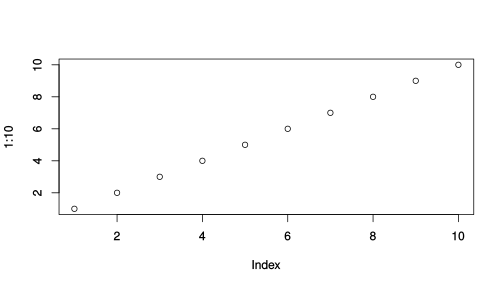
\includegraphics{figs/test/unnamed-chunk-2-1.png}
\caption{plot of chunk unnamed-chunk-2}
\end{figure}


\chapter{Algorithms}
\section{Review of Numerical Methods for Non-Linear Optimizations in Statistics and Related Fields}
\section{Algorithms for Robust Estimators in Statistics}
\section{Propositions}
\input{Rmd/theory_algorithm_nr_rfh}
\input{Rmd/theory_algorithm_fp_rfh}

%------------------------------------------------

\ctparttext{This is the part where I want to introduce the software where the theoretical concepts find implementation.}

\part{Implementation}
\chapter{Verification of Results}
\chapter{Performance of Algorithms, a Statisticians Perspective}
\chapter{Validation of Point Estimates, a Users Perspective}
\chapter{Software}

%------------------------------------------------

\ctparttext{This is the part where I will present all results. Most certainly they will contain a lot of model- and design-based simulation studies for various settings. Maybe there will be more data available and I can present some applications.}

\part{Results}
\chapter{Numerical Accuracy}
\chapter{Stability}
\chapter{Speed of Convergence}
\chapter{Computational Complexity}
\chapter{Simulation Studies}
\section{Area Level Models}
\subsection{The Area-Level Perspective}
\input{Rmd/results_area_level_mc}

\subsection{From Unit to Area Level Data}
\input{Rmd/results_unit_to_area_level_mc}

%----------------------------------------------------------------------------------------
%	THESIS CONTENT - APPENDICES
%----------------------------------------------------------------------------------------

\appendix

\part{Appendix} % New part of the thesis for the appendix

%\include{Chapters/Chapter0A} % Appendix A
%\include{Chapters/Chapter0B} % Appendix B - empty template

%----------------------------------------------------------------------------------------
%	POST-CONTENT THESIS PAGES
%----------------------------------------------------------------------------------------

\cleardoublepage\include{tex/Bibliography} % Bibliography

%\cleardoublepage\include{tex/Colophon} % Colophon

%\cleardoublepage% Declaration

\refstepcounter{dummy}
\pdfbookmark[0]{Declaration}{declaration} % Bookmark name visible in a PDF viewer

\chapter*{Declaration} % Declaration section text

\thispagestyle{empty}

I certify that this work contains no material which has been accepted for the
award of any other degree or diploma in my name, in any university or other
tertiary institution and, to the best of my knowledge and belief, contains no
material previously published or written by another person, except where due
reference has been made in the text.

\bigskip

\noindent\textit{\myLocation, \myTime}

\smallskip

\begin{flushright}
\begin{tabular}{m{5cm}}
\\ \hline
\centering\myName, \today \\
\end{tabular}
\end{flushright}
 % Declaration

%----------------------------------------------------------------------------------------

\end{document}
